\section*{Введение}
\addcontentsline{toc}{section}{Введение}

В настоящей работе рассматривается процесс создания системы управления для умного зала. Такие системы очень востребованы
на сегодняшний день, однако не существует готовых продуктов, которые покрывали бы все требования пользователя.

Таким образом в данной работе разрабатывается ПО, которое решает следующие задачи:
\begin{enumerate}
    \item Удалённое управление электронными устройствами;
    \item Удобное взаимодействие с системой управления через графический интерфейс;
    \item Возможность быстрого и удобного расширения списка поддерживаемых устройств.
\end{enumerate}

Данная работа состоит четырёх частей. В первой части описываются технологии, которые использовались при создании данного ПО
и даются основные понятия, используемые в ходе изложения. Во второй части происходит описание работы приложения с точки
зрения пользователя. В третьей части даётся описание архитектуры всей системы, краткое описание её компонентов, а также способов
взаимодействия между ними. В заключительной четвёртой части реализация компонентов системы рассматривается более подробно.

Результатом этой работы будет служить ПО, которое решает задачу поставленную ранее.

\clearpage

\section{Используемые технологии}

При разработки данного ПО была использована микросервисная архитектура (\ref{def:microservices}), которая в свою очередь
подразумевает использование архитектуры «клиент-сервер» (\ref{def:client-server}).

\begin{definition}
    \label{def:microservices}
    Микросервисная архитектура — вариант архитектуры программного обеспечения,
    ориентированный на взаимодействие насколько это возможно небольших, слабо связанных и легко изменяемых
    модулей — микросервисов.
\end{definition}

\begin{definition}
    \label{def:client-server}
    Архитектура «клиент-сервер» — сетевая архитектура, в которой сетевая нагрузка распределена между поставщиками услуг,
    называемыми серверами, и заказчиками услуг, называемыми клиентами. Обычно клиенты и сервер расположены на разных
    машинах и взаимодействуют между собой через сеть посредством сетевых протоколов (\ref{def:network-protocol}),
    однако они могут быть расположены и на одной машине.
\end{definition}

\begin{definition}
    \label{def:network-protocol}
    Сетевой протокол — набор правил и очерёдности действий, позволяющий осуществлять соединение и
    обмен данными между двумя и более включёнными в сеть устройствами.
\end{definition}

\noindent В качестве серверной части используется ряд микросервисов, которые связаны с клиентской частью посредством
веб-сервера (\ref{def:web-server}), а в качестве клиента используется веб-браузер (\ref{def:web-browser}).

\begin{definition}
    \label{def:web-server}
    Веб-сервер — сервер, принимающий HTTP-запросы от клиентов, обычно веб-браузеров, и выдающий им HTTP-ответы,
    как правило, вместе с HTML-страницей, изображением, файлом, медиа-потоком или другими данными.
\end{definition}

\begin{definition}
    \label{def:web-browser}
    Веб-браузер — прикладное программное обеспечение для просмотра веб-страниц, компьютерных файлов и каталогов,
    управления веб-приложениями, а также для решения других задач.
\end{definition}

\noindent У такого решения существует ряд преимуществ:

\begin{enumerate}
    \item Существует множество реализаций веб-серверов для различных языков программирования.
    Это позволяет использовать уже готовые библиотеки и сосредоточиться непосредственно на написании функционала
    и реализации бизнес-логики.
    \item Использование веб-браузера в качестве клиента позволяет запускать приложение практически на любой платформе:
    десктопе, одноплатных компьютерах, мобильных устройствах, игровых консолях и пр.
    \item Т.к. все вычисления и логика работы выполняются на сервере, то снижаются требования к устройствам, на которых
    запущена клиентская часть приложения.
\end{enumerate}

\noindent Данные между клиентом и сервером, а также между отдельными микросервисами передаются в JSON формате
(\ref{def:json}). Компоненты серверной части общаются между собой по протоколу MQTT (\ref{def:mqtt}).

\begin{definition}
    \label{def:json}
    JSON — текстовый формат обмена данными, основанный на подмножестве языка JavaScript.
\end{definition}

\begin{definition}
    \label{def:mqtt}
    MQTT — упрощённый сетевой протокол, работающий поверх TCP/IP, ориентированный для обмена сообщениями между устройствами
    по принципу издатель-подписчик. 
\end{definition}

\noindent Т.к. клиентская часть реализованна в виде веб-приложения, то для её написания использовался язык программирования
JavaScript (\ref{def:js}), язык разметки HTML (\ref{def:html}) и язык стилей CSS (\ref{def:css}). При общении с сервером
широко применяется технология SSE (\ref{def:sse}).

\begin{definition}
    \label{def:html}
    HTML — cтандартизированный язык разметки документов в сети Интернет.
    Язык HTML интерпретируется браузерами. Полученный в результате интерпретации форматированный текст
    отображается на экране монитора компьютера или мобильного устройства.
\end{definition}

\begin{definition}
    \label{def:css}
    CSS — формальный язык описания внешнего вида документа, написанного с использованием языка разметки.
\end{definition}

\begin{definition}
    \label{def:js}
    JavaScript — мультипарадигменный язык программирования. Поддерживает объектно-ориентированный, императивный и
    функциональный стили. Наиболее широкое применение находит в браузерах как язык сценариев для придания интерактивности
    веб-страницам.
\end{definition}

\begin{definition}
    \label{def:sse}
    SSE (Server-Sent Events) представляет собой технологию отправки уведомлений от сервера к веб-браузеру в виде DOM-событий.
\end{definition}

\noindent Основной функционал серверной части приложения написан на языке Python (\ref{def:python}). Однако для написания
файлов конфигураций использовались и другие языки, например XML (\ref{def:xml}) и YAML (\ref{def:yaml}).

\begin{definition}
    \label{def:python}
    Python — высокоуровневый язык программирования общего назначения, ориентированный на повышение производительности
    разработчика и читаемости кода.
\end{definition}

\begin{definition}
    \label{def:xml}
    XML — расширяемый язык разметки. XML разрабатывался как язык с простым формальным синтаксисом, удобный для создания
    и обработки документов программами и одновременно удобный для чтения и создания документов человеком.
    Язык называется расширяемым, поскольку он не фиксирует разметку, используемую в документах:
    разработчик волен создать разметку в соответствии с потребностями к конкретной области, будучи ограниченным лишь
    синтаксическими правилами языка.
\end{definition}

\begin{definition}
    \label{def:yaml}
    YAML — формат сериализации данных, концептуально близкий к языкам разметки, но ориентированный на удобство
    ввода-вывода типичных структур данных многих языков программирования.
\end{definition}

\noindent Для обеспечения одновременной работы сразу со множеством клиентов серверная часть использует несколько видов
конкурентности (\textit{concurrency}): потоки (\textit{threads}) (\ref{def:thread}) и асинхронный ввод/вывод
(\ref{def:async-io}).

\begin{definition}
    \label{def:thread}
    Поток выполнения — наименьшая единица обработки, исполнение которой может быть назначено ядром операционной системы.
    Реализация потоков выполнения и процессов в разных операционных системах отличается друг от друга, но в большинстве
    случаев поток выполнения находится внутри процесса. Несколько потоков выполнения могут существовать в рамках одного
    и того же процесса и совместно использовать ресурсы, такие как память, тогда как процессы не разделяют этих ресурсов.
\end{definition}

\begin{definition}
    \label{def:async-io}
    Асинхронный ввод/вывод — форма неблокирующей обработки ввода/вывода, которая позволяет процессу
    продолжить выполнение не дожидаясь окончания передачи данных.
\end{definition}

\noindent Микросервисы в серверной части приложения используют технологии виртуализации (\ref{def:virtualization}) и
контейнеризации (\ref{def:containers}). Для автоматического развёртывания и удобства управления контейнерами используется
ПО Docker (\ref{def:docker}).

\begin{definition}
    \label{def:virtualization}
    Виртуализация — предоставление набора вычислительных ресурсов, абстрагированное от аппаратной реализации,
    и обеспечивающее при этом логическую изоляцию друг от друга вычислительных процессов, выполняемых на одном
    физическом ресурсе. 
\end{definition}

\begin{definition}
    \label{def:containers}
    Контейнеризация — метод виртуализации, при котором ядро операционной системы поддерживает несколько изолированных
    экземпляров пространства пользователя вместо одного. Эти экземпляры (обычно называемые контейнерами) с точки зрения
    пользователя полностью идентичны отдельному экземпляру операционной системы.
\end{definition}

\begin{definition}
    \label{def:docker}
    Docker — программное обеспечение для автоматизации развёртывания и управления приложениями в средах с
    поддержкой контейнеризации. Позволяет «упаковать» приложение со всем его окружением и зависимостями в контейнер,
    а также предоставляет среду по управлению контейнерами.
\end{definition}

\clearpage

\section{Описание работы приложения}

Возможности управления, предоставляемые системой напрямую зависят от устройств с которыми она работает. В данном случае
у нас имеется следующий список устройств:

\begin{itemize}
    \item Видеоматрица. Используется для коммутации видеоканалов.
    \item Аудиоматрица. Используется для коммутации аудиоканалов.
    \item Конгресс-система с 12-ю стационарными микрофонами и 2-мя радиомикрофонами.
    \item Видеопроцессор с функцией PIP (Picture-in-Picture).
    \item Терминал видеоконференцсвязи с 2-мя видеокамерами.
    \item 4 телевизора.
    \item Сервер для работы системы управления.
    \item Сенсорный дисплеей, подключенный напрямую к серверу. Любое управление системой осуществляется через него.
\end{itemize}

\noindent Такой набор оборудования позволяет нам совершать групповые видеозвонки, а также проводить локальные или удалённые
совещания и презентации.

\begin{figure}[h]
    \centering
    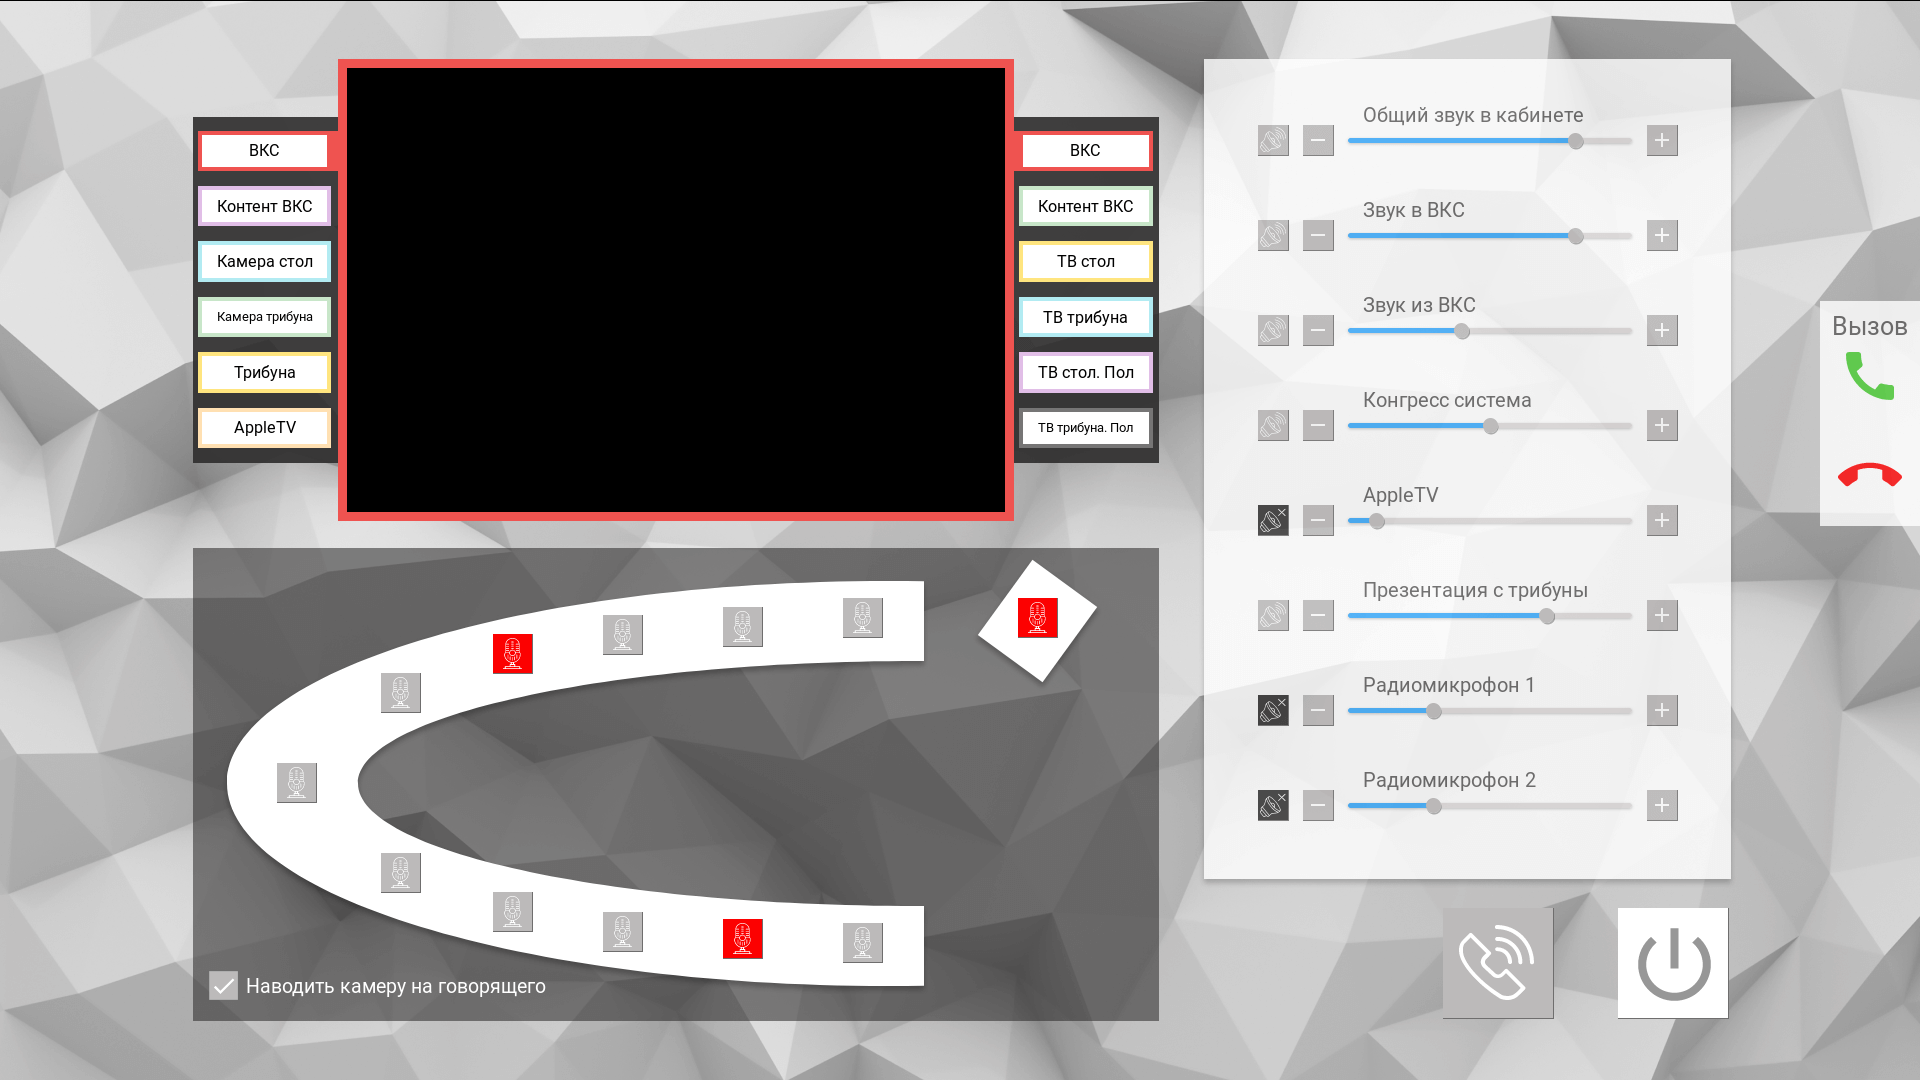
\includegraphics[width=0.8\linewidth]{main_screen.png}
    \caption{Главный экран приложения.}
    \label{fig:main_screen}
\end{figure}

\noindent Для управления данными устройствами был разработан интерфейс, состоящий из 3-х экранов. Главный экран приложения
(рис. \ref{fig:main_screen}) предоставляет основные компоненты для взаимодействия с залом.

\begin{enumerate}
    \item С помощью элемента \textit{видеоматрица} можно управлять входами (слева) и выходами (справа) видеоматрицы.
    Цвет выхода совпадает с цветом входа к которому он привязан в данный момент. Для работы данной функции необходима
    видеоматрица. Также, при нажатии на любой видеовход картинка с него, с помощью функции PIP, начинает выводиться в чёрную
    область элемента.
    \item Элемент с кнопками микрофонов позволяет включить или выключить соответствующий микрофон. Также, при помощи
    соответствующего чекбокса можно перевести камеру в режим автоматического слежения за говорящим. За работу микрофонов
    отвечает конгресс-система.
    \item Слайдеры в правой части экрана позволяют менять громкость звука различных устройств в зале. Для реализации этого
    функционала используется аудиоматрица.
\end{enumerate}

\noindent С помощью кнопки в правом нижнем углу можно попасть на экран для звонков (рис. \ref{fig:dialer_screen}).

\begin{figure}[h]
    \centering
    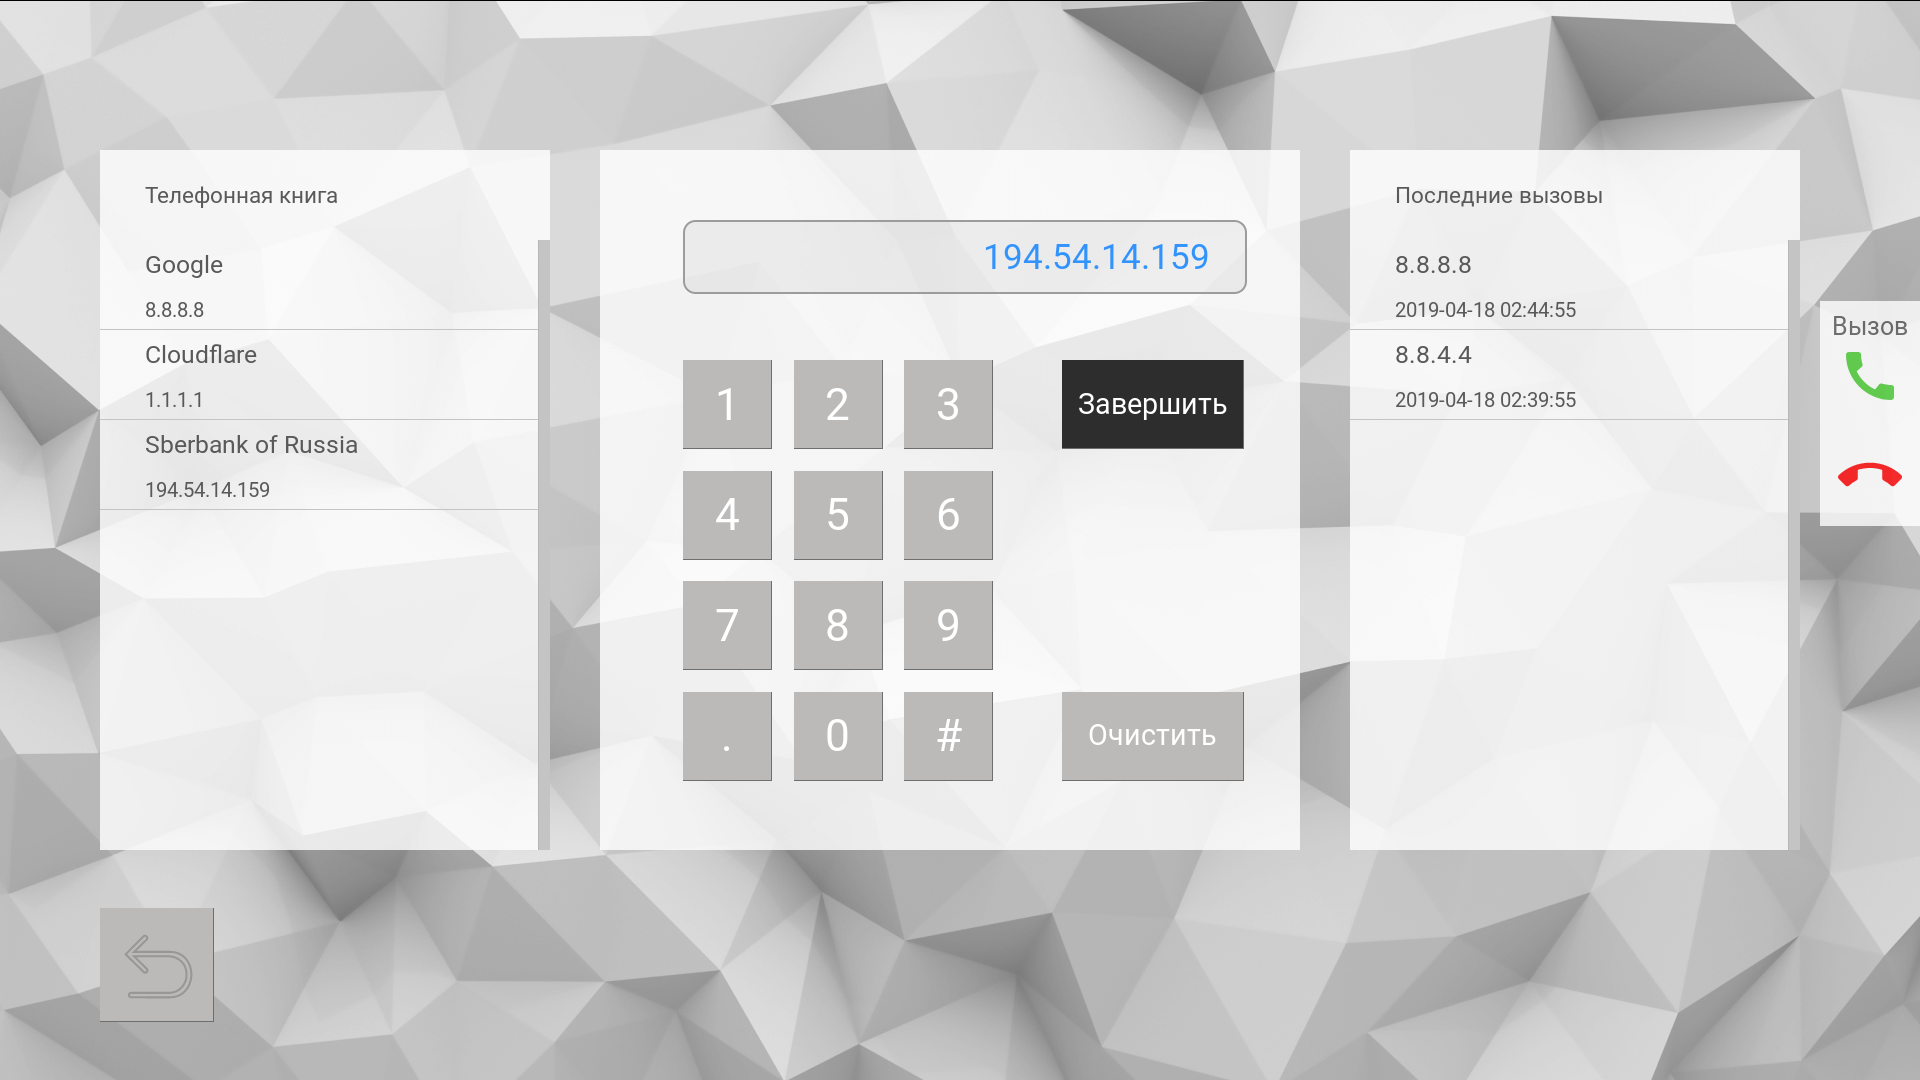
\includegraphics[width=0.8\linewidth]{dialer_screen.png}
    \caption{Экран для совершения видеозвонков.}
    \label{fig:dialer_screen}
\end{figure}

\noindent С данного экрана можно набрать (или выбрать из списка контактов) номер и совершить видеовызов. При этом справа
появится панель с возможностью завершить вызов. Такая же панель появляется при входящем вызове на любом из экранов,
в таком случае кнопками на ней можно принять или отклонить входящий вызов. Вернуться на главный экран можно с помощью
соответствующей кнопки в левом нижнем углу.

~\

\noindent Третий экран приложения отвечает за управление питанием оборудования, а также за различные сценарии использования
конференц-зала (рис. \ref{fig:power_screen}).

\begin{figure}[h]
    \centering
    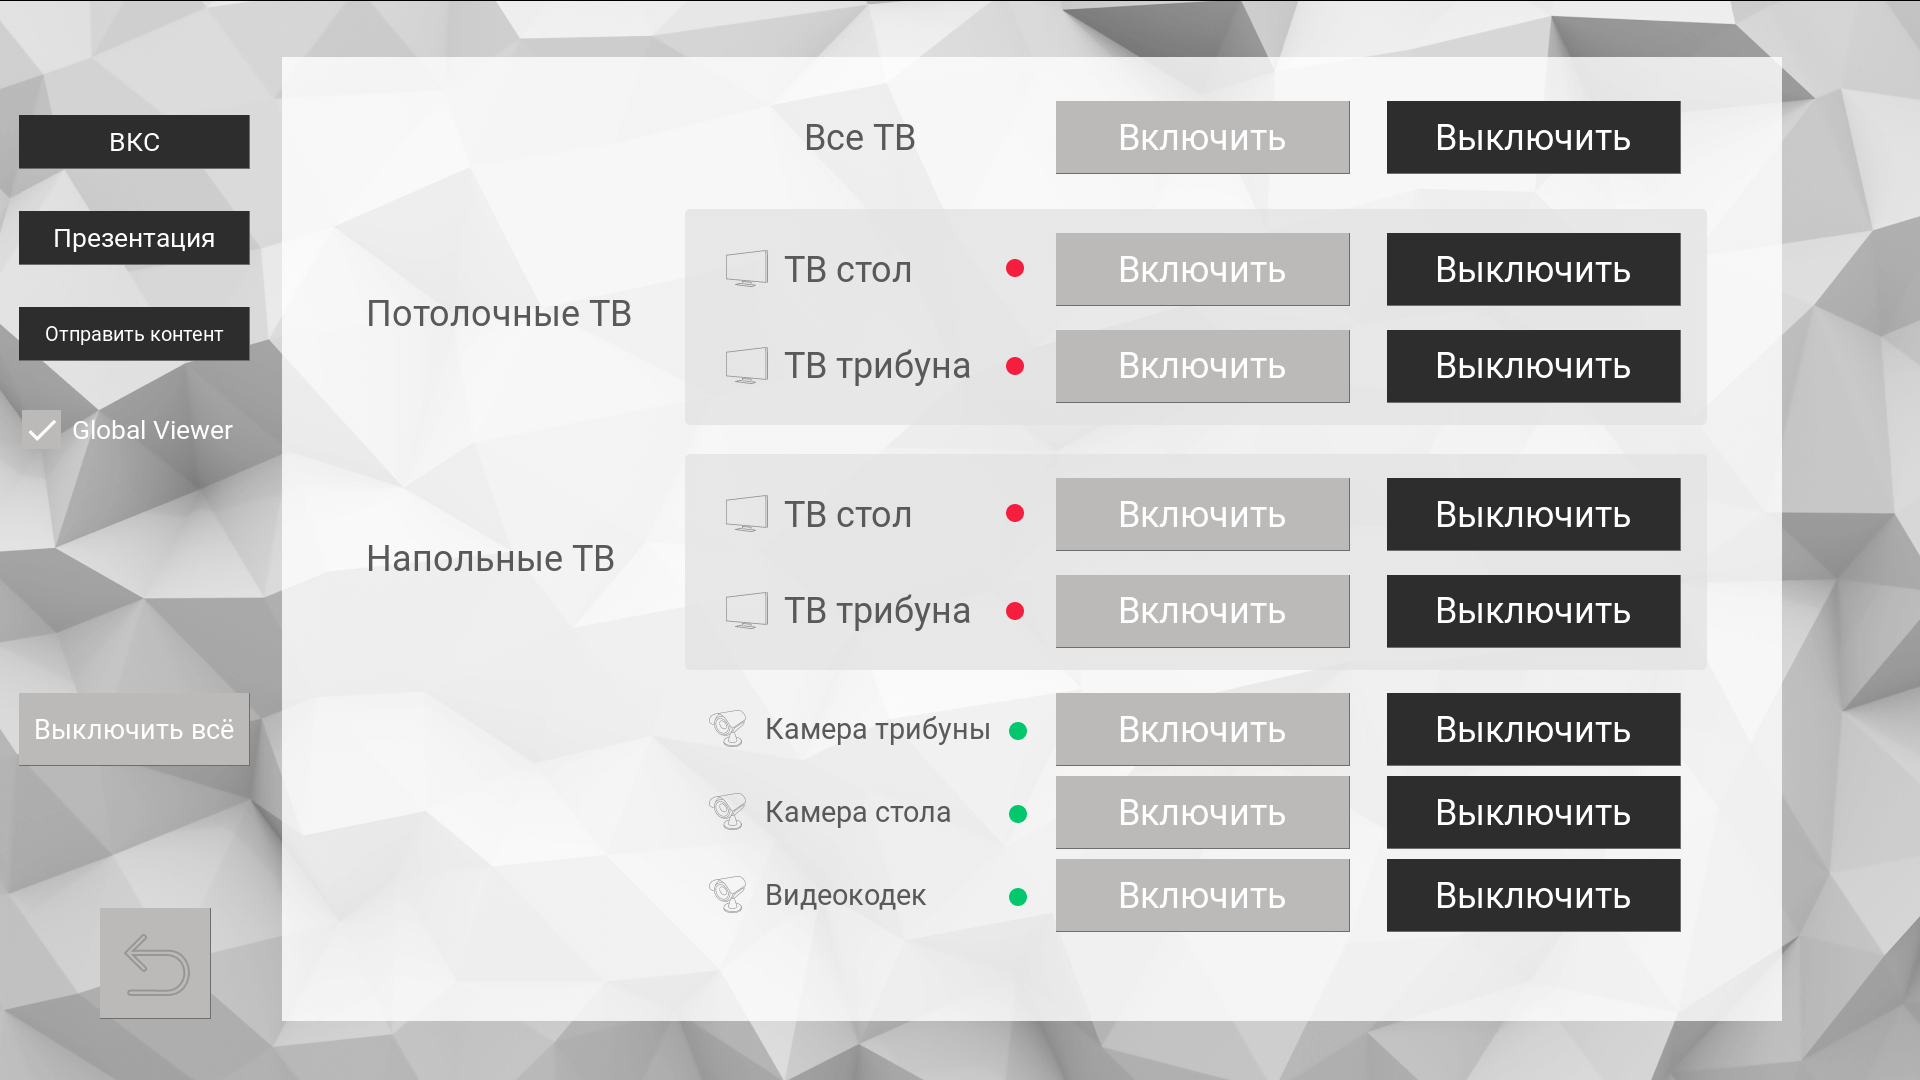
\includegraphics[width=0.8\linewidth]{power_screen.png}
    \caption{Экран для управления питанием устройств.}
    \label{fig:power_screen}
\end{figure}

\noindent Индикаторы показывают текущее состояния оборудования:

\begin{itemize}
    \item Зелёный - устройство работает;
    \item Красный - устройство выключено;
    \item Жёлтый - устройство недоступно.
\end{itemize}

\noindent С помощью кнопок в левом верхнем углу можно включить определённый сценарий
использования зала (например настроить зал для показа презентации или видеозвонка). После нажатия всё оборудование
будет сконфигурировано нужным образом.

~\

\noindent Кнопка \textit{Выключить всё} при нажатии и удержании более 5-ти секунд выключит всё оборудование в зале, в т.ч.
и сервер с системой управления.

\clearpage

\section{Архитектура системы}

Как было сказано ранее данное ПО использует микросервисную архитектуру (\ref{def:microservices}). Каждый компонент системы
предоставляет собой модуль, который работает в Docker-контейнере (\ref{def:docker}) и взаимодействует с другими модулями
по сети. Схема взаимодействия представлена на рис. \ref{fig:arch}.

\begin{figure}[h]
    \centering
    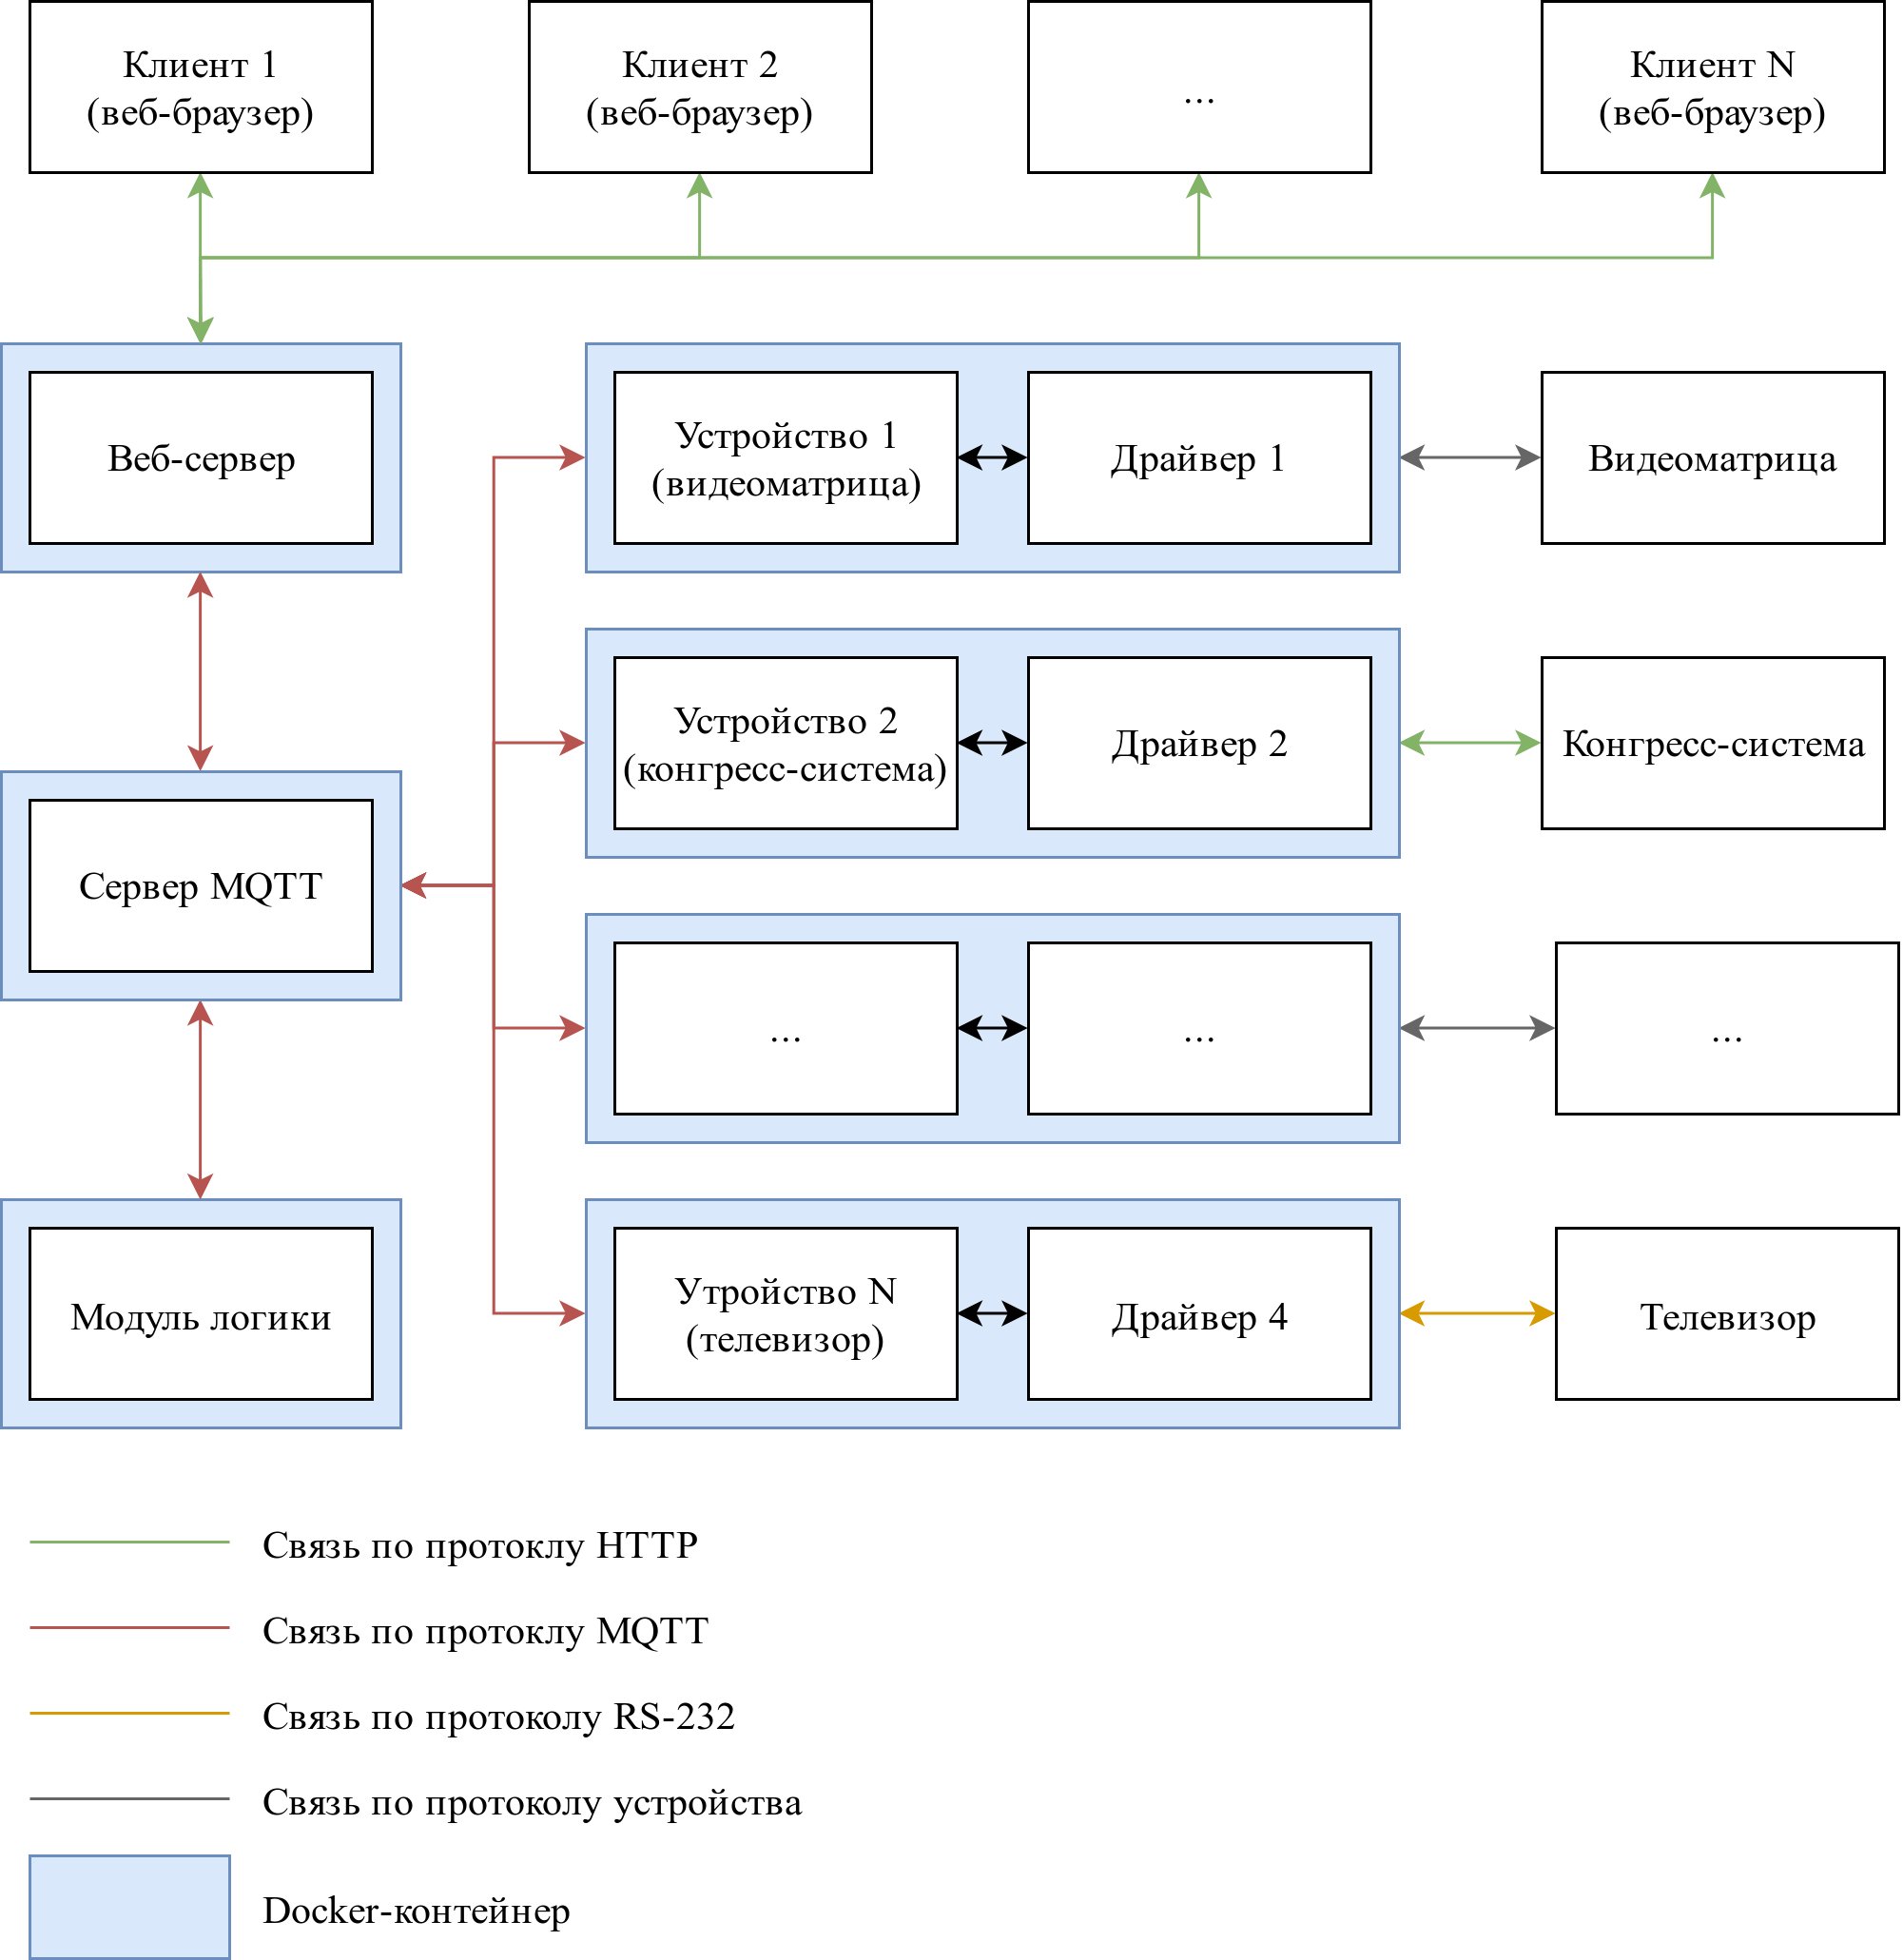
\includegraphics[width=1\linewidth]{arch.png}
    \caption{Схема взаимодействия компонентов системы.}
    \label{fig:arch}
\end{figure}

\noindent Благодаря тому, что компоненты программы общаются друг с другом по сети, приложение может быть запущено как
на одной машине, так и на нескольких (вплоть до того, что каждый Docker-контейнер может быть запущен на отдельном сервере).
Такая распределённая система даёт следующие преимущества:
\begin{enumerate}
    \item \textbf{Производительность и масштабируемость}. При необходимости можно перераспределить нагрузку на сервер
    просто перенеся некоторые из Docker-контейнеров на другой, более мощный компьютер.
    \item \textbf{Отказоустойчивость} - система сохранит частичную или полную работоспособность в случае отказа одного
    или нескольких компонентов.
\end{enumerate}

\subsection{Основные компоненты системы}

Можно выделить следующие основные модули системы:

\begin{itemize}
    \item \textbf{Веб-сервер}. Используется для взаимодействия с веб-браузером. Принимает данные от модуля логики и отдаёт
    их подключенным клиентам.
    \item \textbf{Сервер MQTT}. Через него происходит всё общение межд модулями. Общение осуществляется по модели подписки.
    Например, веб-сервер подписан только на сообщения от модуля логики т.к. принимает команды только от него. Модуль
    логики в свою очередь подписан на все сообщения в системе т.к. ему необходимо знать что происходит между её частями.
    \item \textbf{Модуль логики}. Контролирует всё поведение системы. Любое событие будь то действие пользователя или реакция
    устройства проходит через него.
    \item \textbf{Модуль устройства}. Отвечает за работу с каким-либо устройством (например с телевизором). Знает что умеет
    делать данный тип устройства. Например, видеоматрица может переключать входы и выходы, телевизор может регулировать
    громкость, а терминал видеоконференцсвязи может звонить. Напрямую взаимодействует с драйвером конкретного устройства,
    который превращает абстрактную команду \textit{включить телевизор} в конкретную команду, которую понимает только данная
    модель телевизора. Такой модуль запускается для каждого физического устройства в зале.
\end{itemize}

\subsection{Взаимодействие частей системы}

Компоненты системы общаются между собой по протоколу MQTT (\ref{def:mqtt}) и передают информацию в следующем виде:

\lstinputlisting[caption=Структура запроса.]{request.json}

\lstinputlisting[caption=Структура ответа.]{response.json}

\noindent Значения полей:

\begin{enumerate}
    \item \textit{SENDER\_NAME} - адрес отправителя конкретного запроса или ответа.
    \item \textit{INITIATOR\_NAME} - адрес отправителя первого запроса из этой цепочки (с кого началась обработка события).
    \item \textit{PRIORITY\_LEVEL} - приоритет запроса.
    \item \textit{COMMAND\_ID} - уникальный идентификатор запроса. Повторяется в ответе.
    Используется для привязки ответов, получаемых асинхронно.
    \item \textit{COMMAND\_NAME} - команда.
    \item \textit{EVENT\_NAME} - событие.
    \item \textit{PARAMETERS} - параметры команды или события в формате «ключ-значение».
    \item \textit{DESCRIPTION} - человекочитаемое описание события или ошибки.
    \item \textit{STATUS} - результат выполнения команды.
\end{enumerate}

\noindent Протокол MQTT позволяет подписываться только на определённые сообщения. Для этого у каждого сообщения существует
заголовок (\textit{topic}) в котором можно указать любые данные. Например это может быть имя отправителя/получателя,
группа в которой он состоит и команда/событие которую он послал. Пример заголовка: \textit{>/Зал 1/У окна/TV/Panasonic1/on/}.

\clearpage

\section{Реализация программных модулей}

\subsection{Клиентская часть}

Первое, что видит пользователь приложения это интерфейс (рис. \ref{fig:main_screen}). Для его отрисовки браузер запрашивает
у сервера те элементы, которые должны присутствовать на экране. Для удобства разработки был написан собственный механизм
создания таких интерфейсов, работающий следующим образом. Любой объект на экране состоит из множества простых элементов.
Простые элементы бывают 5 видов: \textit{группа}, \textit{надпись}, \textit{картинка}, \textit{поле для ввода} и
\textit{слайдер}. Комбинируя их в любом количестве мы можем создавать объекты любой сложности. Например, объединив
\textit{надпись} и \textit{группу} можно сделать кнопку с текстом, а если добавить в эту \textit{группу} \textit{картинку},
то будет кнопка с текстом и иконкой.

Вся разметка страницы хранится и передаётся браузеру в формате JSON (\ref{def:json}). После того, как браузер
получил данные от сервера он преобразует эти данные в HTML разметку (\ref{def:html}) для отображения на странице. Этот подход
отличается от более стандартного: веб-сервер отдаёт браузеру готовый HTML код и браузер сразу рендерит страницу.
Данный способ работы был выбран из-за того, что он позволяет создать визуальный редактор интерфейса, который будет работать
прямо в браузере. В случае же с преобразованием JSON в HTML на сервере это привело бы к написанию кода с одинаковой
функциональностью в 2-х различных местах программы.

\subsection{Веб-сервер}

Взаимодействие с браузером происходит через веб-сервер (\ref{def:web-server}) посредством технологии SSE (\ref{def:sse}).
Для его написанния используется язык Python (\ref{def:python}), а также фреймворк \textit{aiohttp}, который работает с
помощью библиотеки для асинхронных вызовов \textit{asyncio}.

Технология SSE позволяет отправлять данные клиентам и отображать их на экране без перезагрузки страницы. Все данные
рассылаются сразу по всем клиентам, подключенным в данный момент. Таким образом любое изменение состояния системы на одном
клиенте приводит к обновлению состояния на всех клиентах.

Для работы сразу с несколькими клиентами веб-сервер использует асинхронный ввод/вывод (\ref{def:async-io}). Это позволяет
создать видимость одновременной работы сразу со всеми клиентами, а также более эффективно использовать время простоя в
моменты передачи данных, что особенно важно в случае веб-сервера.

\subsection{Сервер MQTT}

MQTT сервер также называется «брокер сообщений». С его помощью происходит обмен данными по одноимённому протоколу,
который используется всеми компонентами системы для передачи данных друг другу. В качестве MQTT сервера был выбран
«Eclipse Mosquitto» как наиболее популярный и часто используемый. «Eclipse Mosquitto» разрабатывается той же организацией,
что и сам протокол MQTT, а значит, что он обеспечивает полную его поддержку.

\subsection{Модуль логики}

Все события, получаемые веб-сервером от браузера, он отправляет в модуль логики. Через модуль логики проходят все сообщения
системы, поэтому он всегда знает о текущем состоянии всех компонентов и на основе этого может ими управлять. У этого
модуля 2 основых задачи:
\begin{enumerate}
    \item Работа с файлами разметки экранов, которые отображает веб-браузер;
    \item Реагирование на события приходящие от пользователя или устройств в зале.
\end{enumerate}
Разберём эти пункты более подробно.

Начнём с файлов разметки. Как говорилось ранее, разметка всех страниц, отображаемых в браузере, хранится в формате JSON.
Для более удобной работы с ней используется шаблонизатор \textit{Jinja}. Это позволяет использовать Python-подобные выражения
прямо внутри файла с разметкой. Например, вместо написания большого объёма кода для создания нескольких одинаковых кнопок,
мы можем обернуть код разметки для кнопки в функцию и вызвать её несколько раз в цикле. При запуске системы все шаблоны
генерируются в валидные JSON файлы. После этого модуль логики считывает их и создаёт на их основе объект с разметками
всех страниц системы. При запросе браузером какой-либо страницы, модуль логики через веб-сервер отдаёт ему нужную разметку.

Теперь разберём реагирование на события. Все события в системе можно разделить на 2 вида: события от пользователя и события
от устройств. Для их удобной обработки был разработан функционал, который позволяет привязать какую-либо функцию к событию,
используя декораторы. Такой подход часто используется в различных библиотеках для языка Python, например в \textit{aiohttp}.
Поскольку через модуль логики проходят все генерируемые события это позволяет при их получении отправлять команды любому
модулю в системе. Например, при получении события о выключении телевизора, мы можем послать данные браузеру, чтобы он
отобразил это на экране.

\subsection{Модуль с драйверами устройств}

Для непосредственного управления устройствами в зале модуль логики отправляет команды драйверам этих устройств. Архитектурно
данный модуль содержит набор классов, которые представляют собой какой-то один тип устройств (телевизоры, аудиоматрицы, и пр.).
Каждый класс может отпралвять абстрактные команды для своего типа устройств, например это могут быть команды
\textit{«переключить видеовход»} для телевизора или \textit{«повернуть камеру»} для камеры. Т.к. с классом могут работать
разные модели устройств, то такие абстрактные команды нужно преобразовывать в команды понятные каждой конкретной модели.
Для этого данные классы используют драйверы устройств.

Драйвер представляет собой компонент, который подключается непосредственно к устройству и работает с ним. Подключение к
происходит посредством сети. Подключаясь к устройству драйвер начинает общаться с ним, по протоколу, который оно понимает.
Это могут быть как обычные HTTP запросы, так и собственный протокол устройства. Драйвер выполняет 2 основных задачи:
\begin{enumerate}
    \item Преобразует полученные абстрактные команды в конкретную последовательность байт и отправляет устройству;
    \item Постоянно следит за событиями, которые генерирует само устройство. Это могут быть как подтверждения полуенных
    и обработанных команд, так и события, происходящие от действий пользователя. Например, человек регулирует громкость
    микрофонов, крутя ручку громкости на конгресс-системе, драйвер получает данное событие и отправляет его в модуль логики
    для обработки.
\end{enumerate}

\clearpage

\section{Заключение}

\clearpage

\section{Список источников}

\clearpage

\section{Приложение}
